% ==========================================================
% 3. Conteúdos e Materiais de Referência
% ==========================================================
\chapter{Conteúdos e Materiais de Referência}
\label{cap:materiais}

Nesta seção são apresentados os documentos, planilhas e quadros utilizados atualmente pela Commit Júnior na rotina operacional de gestão de membros, horas e controle disciplinar. Tais registros evidenciam as limitações do modelo manual e fundamentam o levantamento de requisitos do novo sistema.

\section{Itens usados atualmente no contexto}

\begin{figure}[!htbp]
    \centering
    \caption[Planilha de Gerenciamento de Membros e Controle Documental]{Planilha de Gerenciamento de Membros e Controle Documental (Google Sheets)}
    \label{fig:ref-membros}
    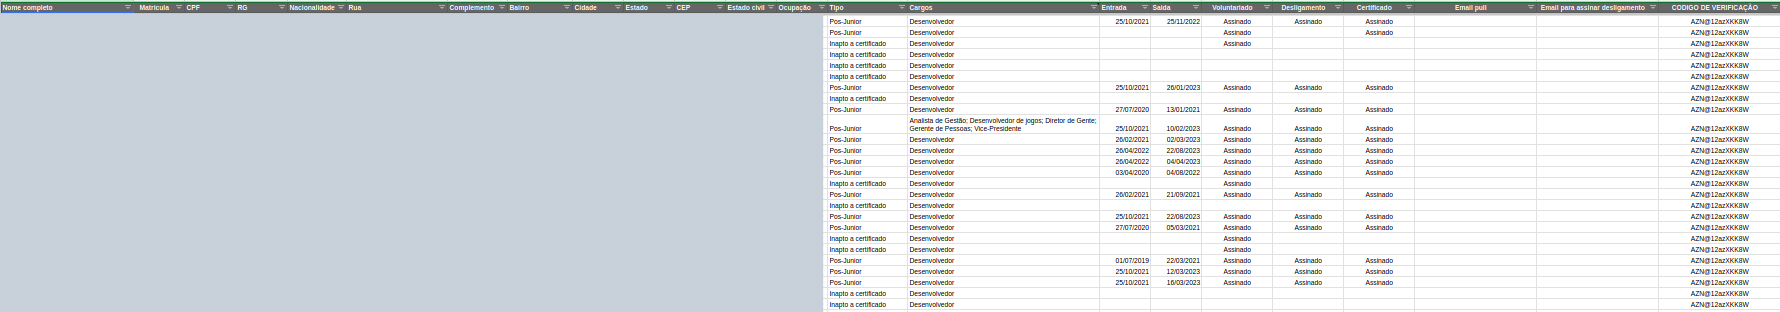
\includegraphics[width=0.95\textwidth]{gerenciamento-de-membros}
\end{figure}
\noindent\textbf{Descrição:} Base gerenciada pelo setor Jurídico e Gestão de Pessoas para controle civil, acadêmico e contratual (termos de voluntariado, desligamento e certificados). Apresenta lacunas de preenchimento, risco de exclusão acidental de linhas e ausência de trilha de auditoria.

\begin{figure}[!htbp]
    \centering
    \caption[Planilha de Gerenciamento e Lançamento de Horas de Extensão]{Planilha de Gerenciamento e Lançamento de Horas de Extensão (Google Sheets)}
    \label{fig:ref-horas}
    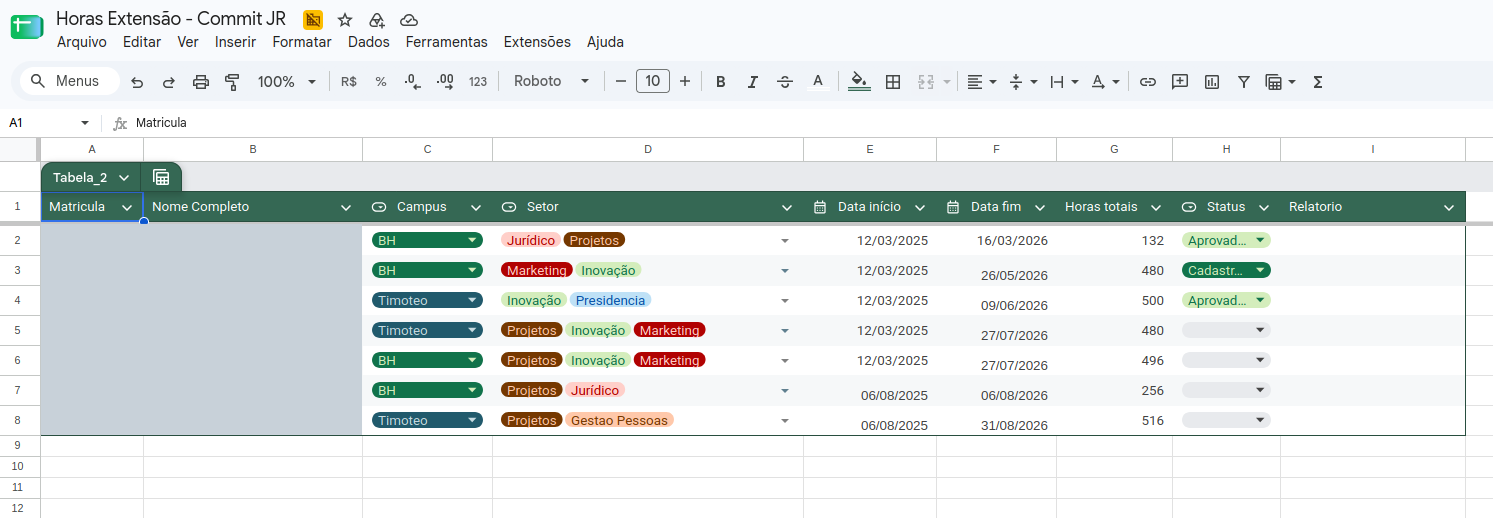
\includegraphics[width=0.95\textwidth]{gerenciamento-de-horas}
\end{figure}
\noindent\textbf{Descrição:} Planilha compartilhada com a coordenação de curso para posterior inserção de horas de extensão no SIGAA. O cômputo do saldo de horas e as notificações de saída de membros dependem de procedimentos manuais e comunicação informal via WhatsApp.

\begin{figure}[!htbp]
    \centering
    \caption[Quadro Geral de Membros e Diretório Corporativo]{Quadro Geral de Membros e Diretório Corporativo (Notion)}
    \label{fig:ref-notion}
    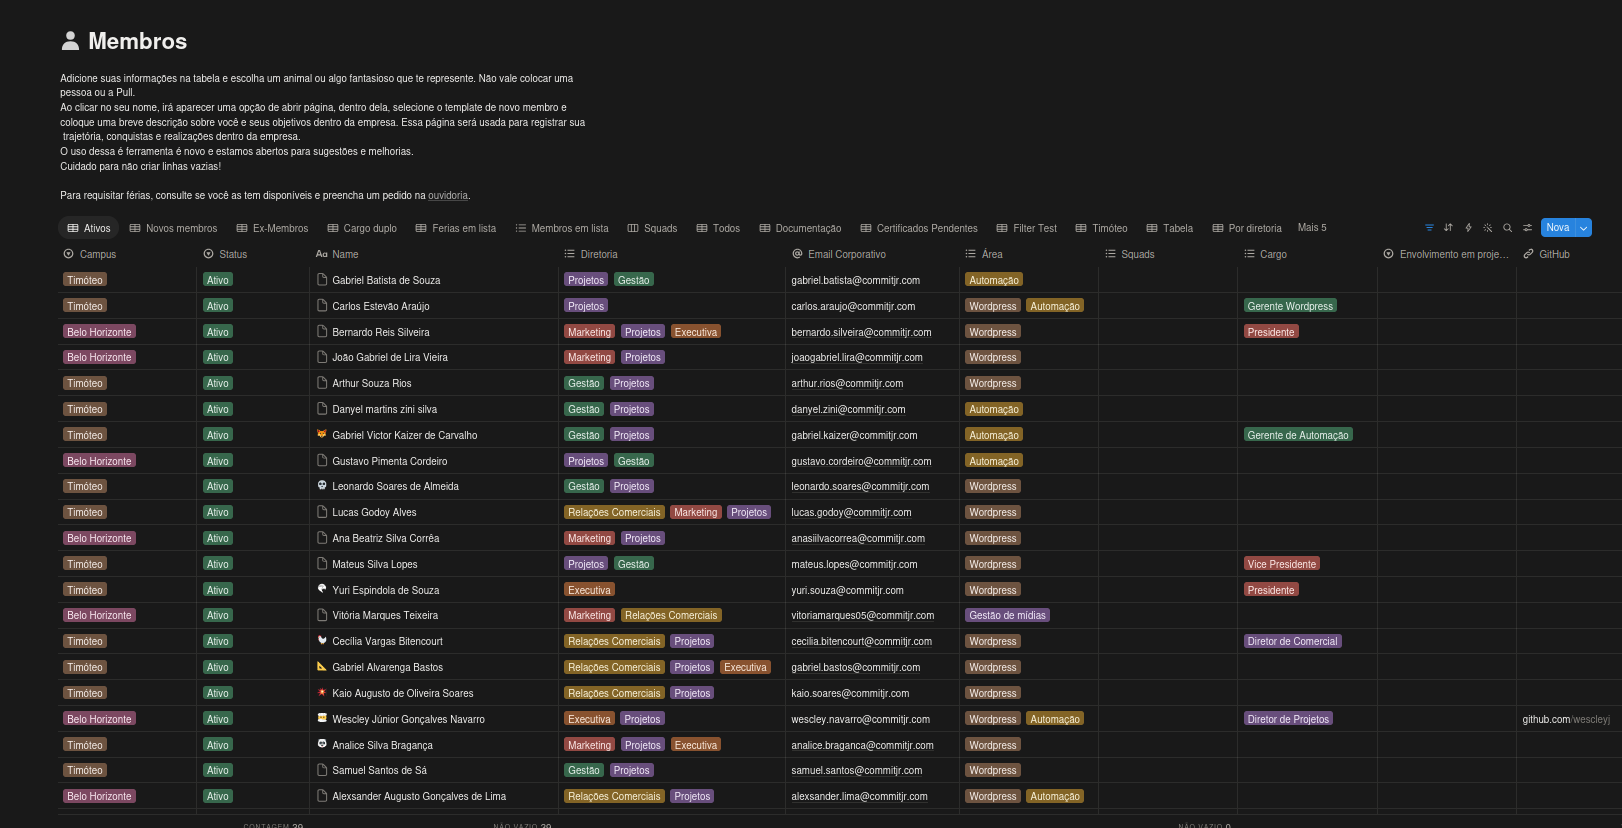
\includegraphics[width=0.95\textwidth]{tela-notion}
\end{figure}
\noindent\textbf{Descrição:} Painel no Notion voltado à consulta interna entre equipes por campus (Timóteo e Belo Horizonte), diretorias, squads e contatos. Sofre com inconsistências cadastrais provocadas pelo esquecimento de atualização e permanência de ex-membros como ativos.

\begin{figure}[!htbp]
    \centering
    \caption[Painel de Lançamento de Pontos e Penalidades]{Painel de Lançamento de Pontos e Penalidades (Notion)}
    \label{fig:ref-pontos}
    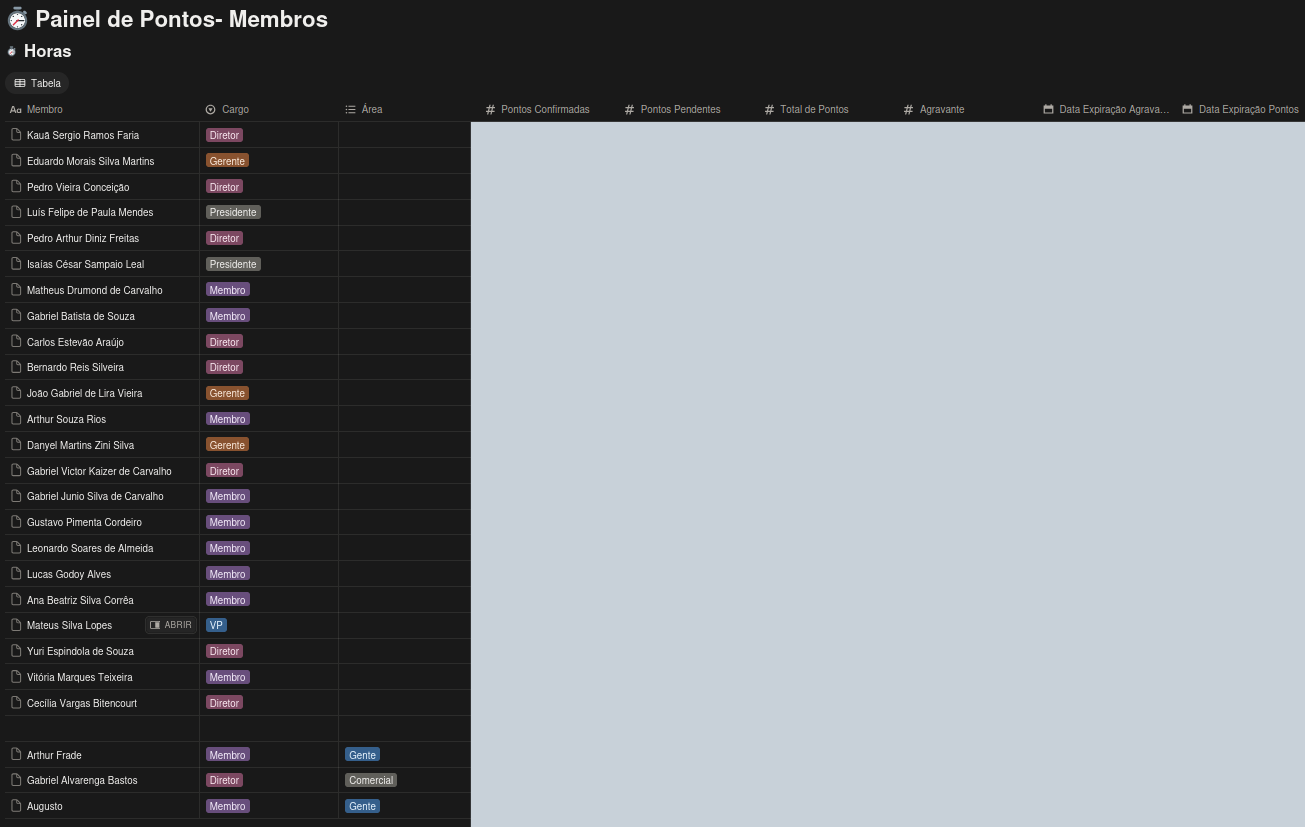
\includegraphics[width=0.95\textwidth]{tela-lancamento-de-pontos}
\end{figure}
\noindent\textbf{Descrição:} Painel para acompanhamento de advertências, agravantes e prazos de validade disciplinar. Possui vulnerabilidade de segurança (permissão aberta para edição por qualquer integrante) e ausência de rotinas automáticas de expiração e reincidência.

\clearpage